
%-=-=-=-=-=-=-=-=-=-=-=-=-=-=-=-=-=-=-=-=-=-=-=-=
%
%        LOADING DOCUMENT
%
%-=-=-=-=-=-=-=-=-=-=-=-=-=-=-=-=-=-=-=-=-=-=-=-=

\documentclass[compress]{beamer}
\usetheme{sthlm}

%-=-=-=-=-=-=-=-=-=-=-=-=-=-=-=-=-=-=-=-=-=-=-=-=
%        LOADING BEAMER PACKAGES
%-=-=-=-=-=-=-=-=-=-=-=-=-=-=-=-=-=-=-=-=-=-=-=-=

\usepackage{
booktabs,
datetime,
dtklogos,
graphicx,
multicol,
pgfplots,
ragged2e,
tabularx,
tikz,
wasysym
}

\pgfplotsset{compat=1.8}
\usepackage[T1]{fontenc}
\usepackage{newpxtext,newpxmath}

\usepackage[utf8x]{inputenc}

\usepackage{multicol}
\usepackage{caption}
\usepackage{pgfgantt}
\usepackage{graphicx} % Allows including images
\usepackage{booktabs} % Allows the use of \toprule, \midrule and \bottomrule in tables

\usepackage{listings}
\lstset{ %
language=[LaTeX]TeX,
basicstyle=\normalsize\ttfamily,
keywordstyle=,
numbers=left,
numberstyle=\tiny\ttfamily,
stepnumber=1,
showspaces=false,
showstringspaces=false,
showtabs=false,
breaklines=true,
frame=tb,
framerule=0.5pt,
tabsize=4,
framexleftmargin=0.5em,
framexrightmargin=0.5em,
xleftmargin=0.5em,
xrightmargin=0.5em
}

%-=-=-=-=-=-=-=-=-=-=-=-=-=-=-=-=-=-=-=-=-=-=-=-=
%        LOADING TIKZ LIBRARIES
%-=-=-=-=-=-=-=-=-=-=-=-=-=-=-=-=-=-=-=-=-=-=-=-=

\usetikzlibrary{
backgrounds,
mindmap
}

%-=-=-=-=-=-=-=-=-=-=-=-=-=-=-=-=-=-=-=-=-=-=-=-=
%        BEAMER OPTIONS
%-=-=-=-=-=-=-=-=-=-=-=-=-=-=-=-=-=-=-=-=-=-=-=-=

\setbeameroption{show notes}

%-=-=-=-=-=-=-=-=-=-=-=-=-=-=-=-=-=-=-=-=-=-=-=-=
%        BEAMER COMMANDS
%-=-=-=-=-=-=-=-=-=-=-=-=-=-=-=-=-=-=-=-=-=-=-=-=


%-=-=-=-=-=-=-=-=-=-=-=-=-=-=-=-=-=-=-=-=-=-=-=-=
%
%	PRESENTATION INFORMATION
%
%-=-=-=-=-=-=-=-=-=-=-=-=-=-=-=-=-=-=-=-=-=-=-=-=
\usepackage{tikz}
\usepackage{pgf}



\logo{
\includegraphics[height=1.5cm]{logo.pdf}}
\newcommand{\nologo}{\setbeamertemplate{logo}{}}

\newcommand{\myquote}[2]{\begin{exampleblock}{}{\large ``#1''}\vskip5mm\hspace*\fill{\small--- #2}\end{exampleblock}}
%----------------------------------------------------------------------------------------
%	TITLE PAGE
%----------------------------------------------------------------------------------------

\title{Hyper-linked Communications} 
\subtitle{WebRTC enabled asynchronous collaboration}


\author{Henrique Rocha} % Your name
\institute[IST] % Your institution as it will appear on the bottom of every slide, may be shorthand to save space
{
Instituto Superior Técnico \\
Universidade de Lisboa \\ % Your institution for the title page
\medskip
\textit{henrique.rocha@tecnico.ulisboa.pt} % Your email address
}
\date{\today} % Date, can be changed to a custom date

\begin{document}
{
\nologo
\begin{frame}
\maketitle % Print the title page as the first slide
\small
Advisor: Ricardo Pereira

Co-Advisor: Paulo Chainho

\end{frame}
}

\begin{frame}[t]
\frametitle{Overview} 
\tableofcontents[hidesubsections]


\end{frame}

%----------------------------------------------------------------------------------------
%	PRESENTATION SLIDES
%----------------------------------------------------------------------------------------

%------------------------------------------------

\section{Introduction}\label{intro}

\begin{frame}[t,shrink]
\frametitle{Introduction} 
\tableofcontents[currentsection,hideothersubsections]

\end{frame}

	\subsection{Context}   % English
		\begin{frame}[c]
		\frametitle{Context}
		Written communication could never replace face to face communication.

		\myquote{No computer in our lifetimes will ever rival a human voice's capacity to conveying rich and complex social and emotional meaning}{Geddes, Martin}

		Today, we can achieve more.
		\end{frame}

	\subsection{Problem Statement} % English
  		\begin{frame}[c]
		\frametitle{Problem Statement}
		Real-time communication applications can make a difference on business, education and health sectors.

		\vfill

		An application that provides a way to remember our past communications would be a strong tool.
		
		\end{frame}


  		\begin{frame}[c]
		\frametitle{Problem Statement: Use case}
		A teacher record and streams an interactive class, some students participate in real-time others may participate later.
		\vfill
		The teacher adds information to its class (create tags, add links, overlay images ...).
		\vfill
		Students can answer to quizzes.
		\end{frame}



		
	

	\subsection{Thesis Goals} % English
  		\begin{frame}[c]
		\frametitle{Thesis Goals}
		Development of an application that applies the hypermedia concepts.

		\vfill
		
		Record and playback interactive video.
		
		\vfill

		Use only standard technologies like JavaScript, WebRTC, HTML5 and CSS3.

		\end{frame}


\section{Related Work}\label{related}

\begin{frame}[t,shrink]
\frametitle{Related Work} 
\tableofcontents[currentsection,hideothersubsections]

\end{frame}

	\subsection{Early days of the Internet}\label{early}


  		\begin{frame}[c]
		\frametitle{Early days of the Internet}
		\begin{itemize}
		\item IPv4 Address Exhaustion
		\vfill
		\item Network Address Translation	
		\vfill
		\item Client-Server model
		\vfill
		\item STUN + TURN = ICE
		\end{itemize}
		\begin{flushright}

			\vspace*{-8\baselineskip}
			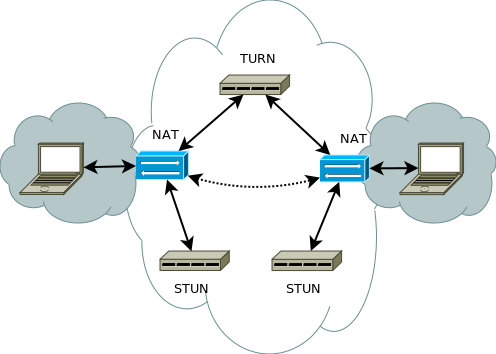
\includegraphics[width=0.55\textwidth]{figures/ice2.png}
		\end{flushright}
		
		\end{frame}




	\subsection{Real-Time communications}\label{rtc}


		\begin{frame}[c]
		\frametitle{Real-Time communications}
		\begin{figure}
			
\includegraphics[height=0.2\textwidth]{figures/skype.png}
			
\includegraphics[height=0.1\textheight]{figures/space.png}
			
\includegraphics[height=0.2\textwidth]{figures/hangouts.png}
			
\includegraphics[height=0.1\textheight]{figures/space.png}
			
\includegraphics[height=0.2\textwidth]{figures/jitsi.png}
		\end{figure}
		\end{frame}

		\begin{frame}[c]
		\frametitle{Real-Time communications}

		WebRTC (Web Real-Time Communications)

		\begin{itemize}
		\item MediaStream	
		\item DataChannel
		\item RTCPeerConnection
		\end{itemize}

		\begin{flushright}

			\vspace*{-5\baselineskip}
			
\includegraphics[width=0.2\textwidth]{figures/webrtc.png}
			
\includegraphics[width=0.2\textwidth]{figures/space.png}
		\end{flushright}
		
		\end{frame}



	\subsection{Signaling}
  		\begin{frame}[c]
		\frametitle{Signaling: meet and get to know}
		\begin{itemize}
		\item Own Implementation
		\vfill
		\item SIP
		\vfill
		\item XMPP
		\vfill
		\item SigOFly 
		\end{itemize}
		\end{frame}



	\subsection{Hypermedia}
  		\begin{frame}[c]
		\frametitle{Hypermedia: more than words, more than images}
		\begin{itemize}
		\item \textbf{Concepts:} HyperText \& HyperMedia \& HyperCommunications
		\vfill
		\item \textbf{Implementations:} HyperCafe \& HyperHitchcock  % Detail on Demand
				
		\end{itemize}
		
		\begin{figure}
			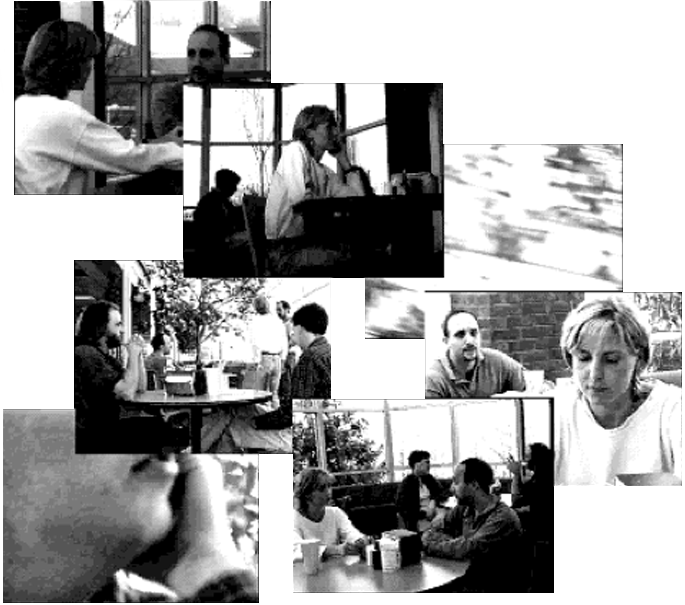
\includegraphics[height=0.4\textheight]{figures/hypercafe.png}
			
\includegraphics[height=0.1\textheight]{figures/space.png}
			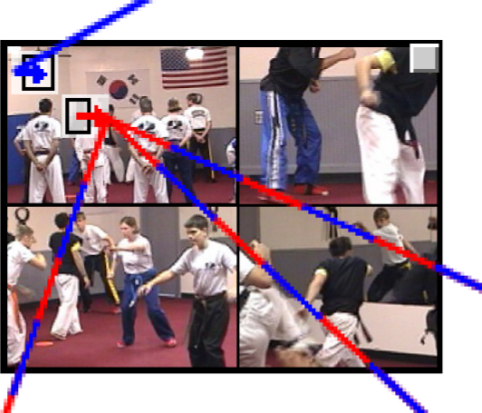
\includegraphics[height=0.4\textheight]{figures/hitchcock.png}
		\end{figure}
		\end{frame}


		\begin{frame}[c]
		\frametitle{Hypermedia: more than words, more than images}
		\begin{itemize}		
		\item \textbf{Languages:} HyVAL \& SMIL
		\vfill
		\item \textbf{WebBrowser:} Ambulant \& SmillingWeb \& SVG
		\end{itemize}
		
		\begin{multicols}{2}
		\begin{figure}
			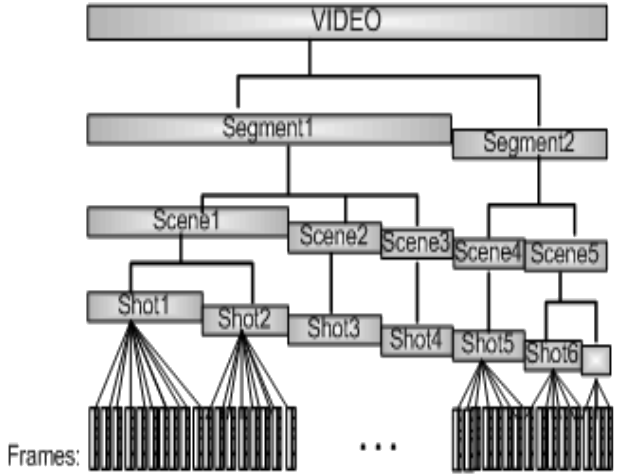
\includegraphics[height=0.4\textheight]{figures/hyval.png}
			\caption{HyVAL structure}
		\end{figure}
		\begin{figure}
			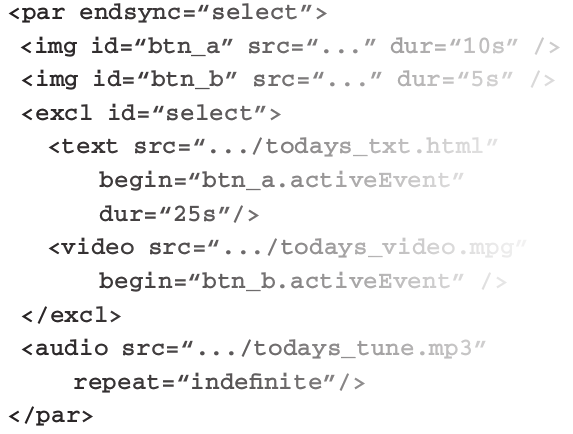
\includegraphics[height=0.4\textheight]{figures/smil.png}
			\caption{SMIL example}
		\end{figure}
		\end{multicols}
		\end{frame}


 		\begin{frame}[c]
		\frametitle{Web-Browser plug-ins}
		\begin{figure}
			
\includegraphics[height=0.3\textheight]{figures/flash.jpg}
			
\includegraphics[height=0.1\textheight]{figures/space.png}
			
\includegraphics[height=0.3\textheight]{figures/silverlight.png}
		\end{figure}
		\end{frame}


	\subsection{Collaboration \& Time manipulation}
  		\begin{frame}[c]
		\frametitle{Extending collaboration tools with time manipulation}
		
		\begin{figure}
			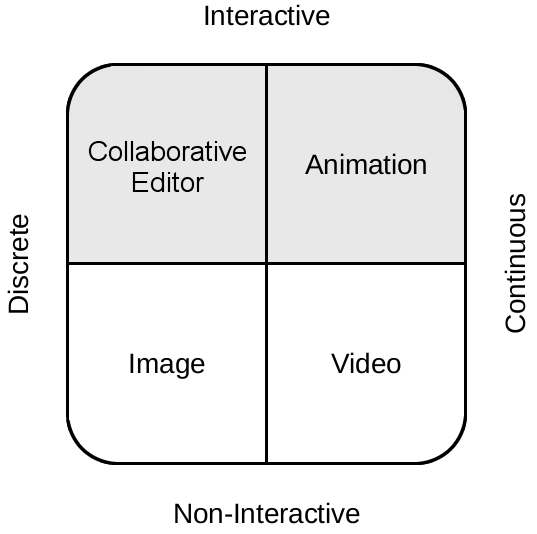
\includegraphics[height=0.5\textheight]{figures/media_types.png}
			\caption{Media Types}
		\end{figure}
		\end{frame}



  		\begin{frame}[c]
		\frametitle{Extending collaboration tools with time manipulation}
		\begin{itemize}
		\item Streaming and Recording (RTP, SRTP)
		\vfill
		\item Recording and Streaming Interactive Media
		\vfill
		\item Collaborative Environment (TogetherJS)
		\end{itemize}
		\end{frame}

%\subsubsection{Streaming and Recording}\label{recstream}
%\subsubsection{Media Types}\label{mediatype}
%\subsubsection{Recording and Streaming Interactive Media}\label{intrecord}
%\subsubsection{Collaborative Environment}\label{collabenv}



\section{Proposed Architecture}\label{arch}

\begin{frame}[t,shrink]
\frametitle{Related Work} 
\tableofcontents[currentsection,hideothersubsections]
\end{frame}

\subsection{Modules}

	\begin{frame}[c]
		\frametitle{Modules}
		\begin{figure}[H]
			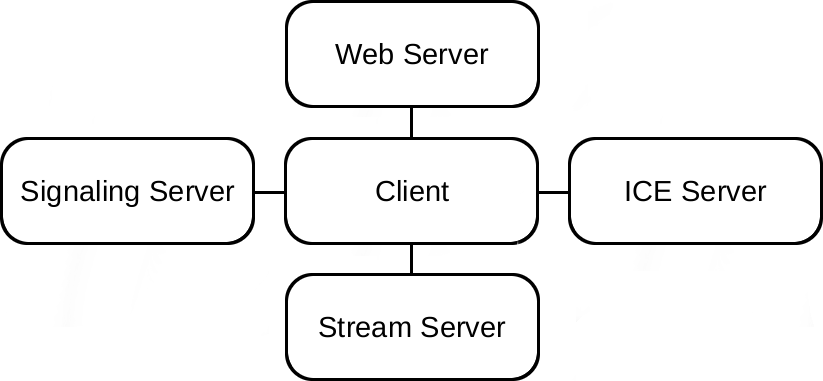
\includegraphics[width=0.6\textwidth]{figures/archs.png}
			\caption{System Modules}
		\end{figure}
	\end{frame}

\subsection{Implementation Proposal}

		\begin{frame}[c]
		\frametitle{Implementation Proposal}


\begin{columns}[c]
\begin{column}{.4\textwidth}
		\begin{figure}[H]
			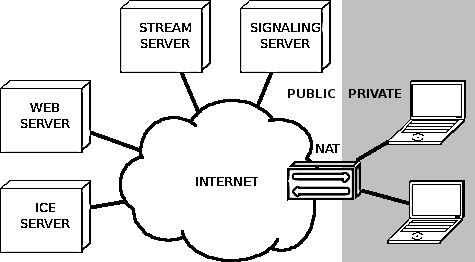
\includegraphics[width=\textwidth]{figures/arch.png}
			\caption{System Infrastructure}
		\end{figure}
\end{column}
\begin{column}{.6\textwidth}

\begin{itemize}
\small
		\item \textbf{ICE Server}: restund
		\vfill
		\item \textbf{Signaling Server}: Ejabberd
		\vfill
		\item \textbf{Web Server}: Play Framework
		\vfill
		\item \textbf{Stream Server}: Jitsi VideoBridge
		\end{itemize}

\end{column}
\end{columns}



{
		\centering
		\begin{figure}[H]
			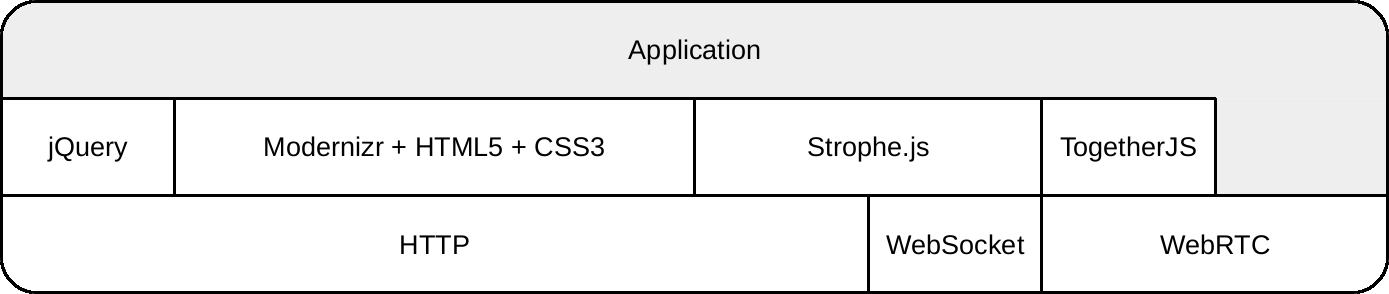
\includegraphics[width=0.9\textwidth]{figures/apparch.png}
			\caption{App Architecture}
		\end{figure}
}

		\end{frame}


\begin{frame}[c]
		\frametitle{Wireframe}
		\begin{figure}[H]
			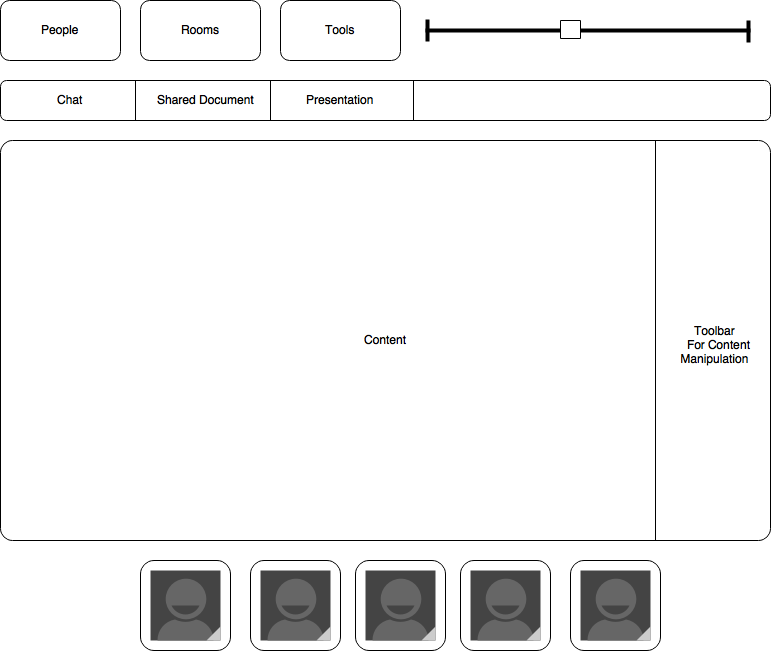
\includegraphics[width=0.6\textwidth]{figures/pbf.png}
			\caption{Application wireframe}
		\end{figure}
	\end{frame}

\section{Methodology}\label{meth} % Section
\subsection{Evaluation}
\begin{frame}[t,shrink]
\frametitle{Related Work} 
\tableofcontents[currentsection,hideothersubsections]
\end{frame}
\begin{frame}[c]
		\frametitle{Evaluation}
Qualitative and quantitative evaluation.

		\begin{itemize}
		\item Tests with users.
		
			\begin{itemize}
			\item Task duration.
			\item Feedback.
			\end{itemize}
		\item Benchmarks.
			\begin{itemize}
			\item Amount of users.
			\item Parallel conversations.
			\end{itemize}
		
		\end{itemize}
	\end{frame}



\subsection{Planned Schedule}
\begin{frame}[c]
\centering
		\frametitle{Planned Schedule}

\tikzset{every picture/.style={xscale=0.35,yscale=0.28,transform shape}}

\begin{ganttchart}[vgrid, hgrid]{1}{36}
\gantttitle{2015}{28}
\gantttitle{2016}{8} \\
\gantttitle{Jun}{4}
\gantttitle{Jul}{4}
\gantttitle{Aug}{4}
\gantttitle{Sep}{4}
\gantttitle{Oct}{4}
\gantttitle{Nov}{4}
\gantttitle{Dec}{4}
\gantttitle{Jan}{4}
\gantttitle{Feb}{4} \\
\gantttitlelist{1,...,36}{1}\\
%First Group
\ganttgroup{Thesis}{1}{35} \\
\ganttbar{Related work evaluation}{1}{30}\\
\ganttbar{Thesis writing}{19}{35} \\
\ganttbar{Paper writing}{25}{35} \\
\ganttmilestone{Delivery}{35}{35} \\
%\ganttlink{elem0}{elem1}
%\ganttgroup{Resume}{1}{10} \\

%\ganttmilestone{Milestone 1}{11}
%Second Group
\ganttgroup{Implementation}{1}{1}\ganttgroup{}{4}{8}\ganttgroup{}{11}{26}\ganttgroup{}{29}{30} \\
\ganttbar{Basic configuration}{1}{1} \\
%\ganttlink{elem4}{elem5}
%\ganttmilestone{Milestone 1}{11}
%Third Group
\ganttbar{WebRTC basics}{4}{4} \\
\ganttbar{Video \& Audio Communication}{4}{5} \\
\ganttbar{Non-Interactive Record \& Playback}{6}{8} \\
\ganttbar{Interactive Record \& Playback}{11}{14}\\
\ganttmilestone{First Prototype}{18}\\
\ganttbar{Collaborative Environment}{15}{18}\\
\ganttmilestone{Second Prototype}{22} \\
\ganttbar{Interface Improvement I}{19}{22} \\
\ganttbar{Usability Tests I}{23}{23} \\
\ganttmilestone{Third Prototype}{25} \\
\ganttbar{Interface Improvement II}{24}{25} \\
\ganttbar{Usability Tests II}{26}{26} \\
\ganttbar{Performance Tests}{29}{30} \\
\ganttbar{Performance Improvements}{30}{30} \\
\ganttmilestone{Final Prototype}{30}

%\ganttlink{elem8}{elem9}


\ganttlink{elem9}{elem10}
\ganttlink[link type=F-S]{elem11}{elem12}
\ganttlink{elem12}{elem13}
\ganttlink[link type=F-S]{elem13}{elem15}
\ganttlink[link type=F-S]{elem15}{elem17}
\ganttlink[link type=F-S]{elem17}{elem18}
\ganttlink[link type=F-S]{elem18}{elem20}
\ganttlink[link type=F-S]{elem20}{elem21}
\end{ganttchart}

	\end{frame}




\section{Conclusions}\label{concl} % English
\begin{frame}[t,shrink]
\frametitle{Related Work} 
\tableofcontents[currentsection,hideothersubsections]
\end{frame}

\begin{frame}[c]
		\frametitle{Conclusions}
		\begin{itemize}
\item New usage scenarios for communication and collaboration applications.
		\vfill

\item Enrich communications using hypermedia concepts. Record, playback and collaboration features.
		\vfill

\item Prototype implementation and testing.
		\end{itemize}

	\end{frame}



%------------------------------------------------

%------------------------------------------------

%------------------------------------------------

\begin{frame}[c]
\Huge{\centerline{Questions?}}
\end{frame}

%----------------------------------------------------------------------------------------

\end{document} 
